% Chapter 5

\chapter{Neural Network Design and Implementation} % Main chapter title

\label{Chapter5} % For referencing the chapter elsewhere, use \ref{Chapter5} 

%----------------------------------------------------------------------------------------
\section{External libraries}
DeepMiRNA has been developed using \emph{Python3}. The \emph{requirements.txt} file, present in the project root directory, contains names and versions of all libraries used for the implementation. In particular, we used \emph{Pandas} and \emph{Numpy} for the preprocessing step and the datasets preparation together with \emph{RNA} (the Python version of the Vienna Cofold) and \emph{Biopython} to parse .fasta files and convert them to .csv. 

Implementation of the neural network was done with \emph{Keras}\cite{keras} using \emph{Tensorflow} backend\cite{tensorflow}. Keras is an open-source neural-network library capable of running on top of TensorFlow, Theano and other major deep learning frameworks. Keras contains numerous implementations of commonly used NN building blocks such as layers, optimizers or activation functions and it aims at being user-friendly, modular and extensible. However, Keras, which is now fully supported in the Tensorflow's core library, has been conceived more as an interface than a standalone framework. 

We opted for the use of this library because it offers a higher-level, more intuitive set of abstractions that makes it easier to develop deep learning models.    

\section{Choosing the right model}
Building deep learning applications in the real world is a never-ending process of selecting and refining the right elements for a specific solution. Among those elements, the selection of the correct model and the right structure of the training dataset are, arguably, the two most important decisions that any data scientist needs to make when designing deep learning solutions. How to decide what deep learning model to use for a specific problem? How do we know whether we are using the correct training dataset or we should gather more data? Those questions are the common denominator across all stages of the life cycle of a deep learning application. Even though there is no magic answer to those questions, there are several ideas that could guide the decision process. 

First of all, we need to start identifying the correct baseline model, in particular, we should select what type of networks suits more the input dataset. In the case of miRNA target predictions, the topological structure of the available data is strictly correlated to the vectorization method selected. If we opt for the one-hot encoding that maps duplexes into fixed-size vectors, we should be thinking of using an MLP network with interlayer connectivity. While, if we select the Dna2Vec approach that transforms each duplex into a matrix, then the problem could be tackled using convolutional neural networks (CNN)\cite{dl}.  

The second part concerns the selection of the optimization algorithm to use. The most popular are, arguably, SGD (Stochastic Gradient Descent) and its variation using momentum or learning decay, and Adam. The latter, in particular, is very often used combined with CNN.

As mentioned in chapter \ref{Chapter4} DeepMiRNA uses 2 different neural networks for the training stage according to the chosen data representation: a regular feed-forward network for the one-hot encoded sequences and a CNN for the Dna2Vec encoded duplexes. 

\section{The feed-forward network} 
The MLP network we designed for the miRNA target prediction task is a very simple neural network consisting of 5 dense hidden layers, comprising rectifier activation function ReLU nodes, each followed by a dropout layer. Dropout \cite{dropout} is a regularization technique used to prevent overfitting. In this thesis, the dropout rate has been set to $0.7$ meaning that there is a probability $p = 0.3$ that a certain neuron is ignored (i.e set to 0). Basically, this implies that their contribution to the activation of downstream (i.e. next layer) neurons is temporally removed on the forward pass and weight update is not applied on the backward pass (see figure \ref{fig:dropout}).

\begin{figure}[hbt!]
	\centering
	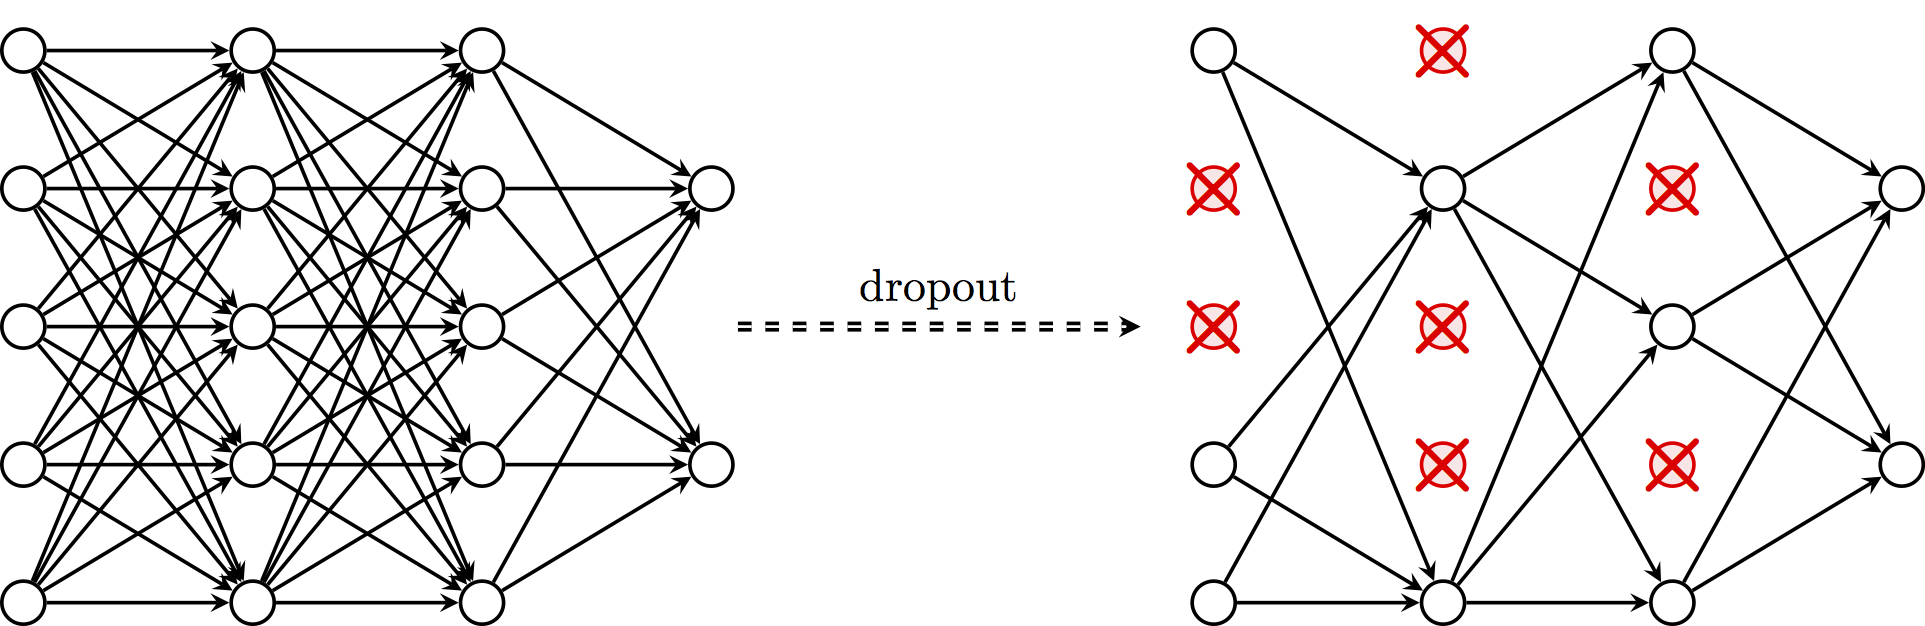
\includegraphics[width=\textwidth, height=0.3\textheight]{Figures/dropout}
	\caption{\keyword{Dropout.} Left: neural network before dropout. Right: neural network after dropout.}
	\label{fig:dropout}
\end{figure}   

While a neural network learns, neuron weights settle into their context within the network. Those weights are tuned for specific features providing some specialization. However, neighboring neurons become to rely on this specialization, which, if taken too far, can result in a fragile model with a reduced generalization capability. Hence, if neurons are randomly dropped out of the network during training, other neurons will have to step in and handle the representation required to make predictions for the missing neurons. This is believed to result in multiple independent internal representations being learned by the network. The effect is that the network becomes less sensitive to the specific weights of neurons and results in a model capable of better generalization and less likely to overfit the training data.    

The output layer is composed of one sigmoid node that returns a value between 0 and 1 corresponding to the final score prediction. The class of the site is determined by the output of this neuron:

\[class(i) = 
\begin{cases} 
	1 & \text{if } o \geq 0.4 \\
	0 & \text{if } o < 0.4
\end{cases}
\]

Where $i$ and $o$ denote respectively the input and the output of the network. The prediction threshold value $0.4$ has been empirically evaluated. 


\begin{figure}[hbt!]
	\centering
	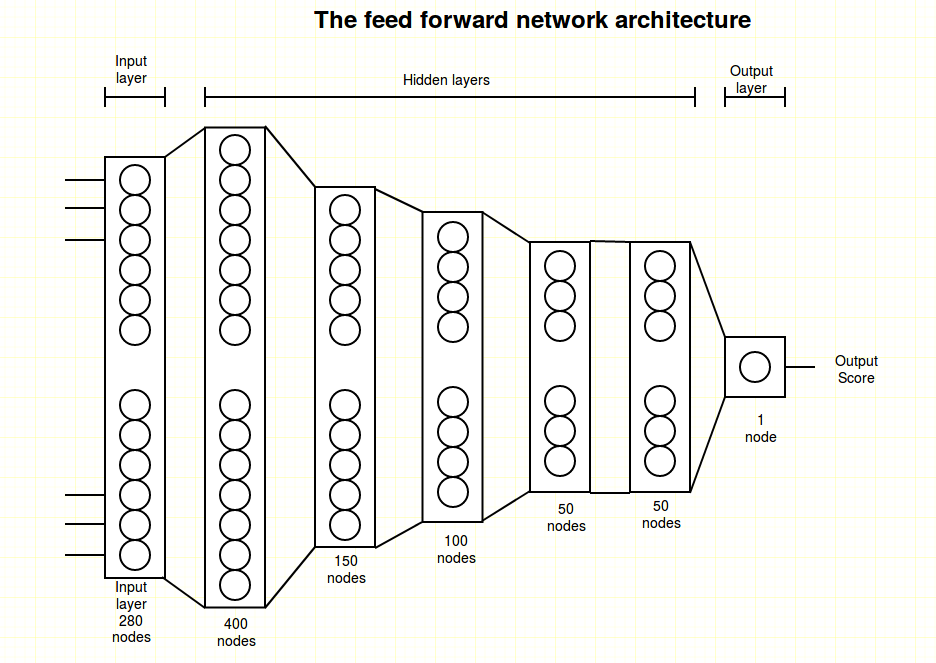
\includegraphics[width=\textwidth, height=0.52\textheight]{Figures/NN}
	\caption{\textbf{The feed-forward neural network}. The first hidden layer increases the dimensionality of the input allowing the representation of data in a more complex feature space. There is a debate in the machine learning community regarding the need for such over-completion layers, as they do not necessarily improve the accuracy whilst making the learning process slower. Considering that the relatively low number of inputs of the proposed network allows a fast training procedure, we opted to include this higher dimension layer to give the network the chance of identifying more complex patterns.}
	\label{fig:NN}
\end{figure}

As loss function, we chose the binary cross entropy with Adam optimizer set with the following parameters:

\begin{itemize}
	\item learning rate = 0.002;
	\item beta\_1 = 0.9;
	\item beta\_2 = 0.999;
	\item epsilon = $1e-8$;
	\item decay = 0.0
\end{itemize}

The resulting architecture can be visualized in figure\ref{fig:NN} and parameters, such as the number of layers and neurons, have been chosen through cross-validation.

Despite being a very simple model, this network showed better performances on the test set compared to other deeper (that is with more hidden layers) or more complex (i.e with a greater number of nodes) models. Check chapter \ref{Chapter6} for further details on the results.

\section{The Convolutional Neural Network aka CNN}
We have explained earlier, that the second encoding function provided by DeepMiRNA is based on Dna2Vec \cite{dna_distributed_repr}. In computational biology, one of the most widely used representations for long DNA sequences consists in dividing the transcript into shorter k-mer components.  Unfortunately, the straightforward vectorization of k-mer as a one-hot vector is vulnerable to the curse of dimensionality. Worse yet, the distance between any pair of one-hot vectors is equidistant, even though, for example, the sequence \emph{ATGGC} should be closer to \emph{ATGGG} than \emph{CACGA}. This might be particularly problematic when applying the latest machine learning algorithms to solve problems in biological sequence analysis. Dna2Vec is, thus, a distributed representation of biological sequences that allows mapping k-mers to dense vectors of real numbers. By splitting the miRNA:MBS duplex in a fixed number of variable length k-mers, we were able to encode each pair into a bi-dimensional matrix. 

More specifically, each k-mer is embedded into a continuous vector space of $100$ dimensions, and each duplex is divided into 9 variable length k-mers: concatenating these vectors we obtain a $9x100$ matrix representing the encoded sequence (see figure \ref{fig:dna_embedding}).

\begin{figure}[hbt!]
	\centering
	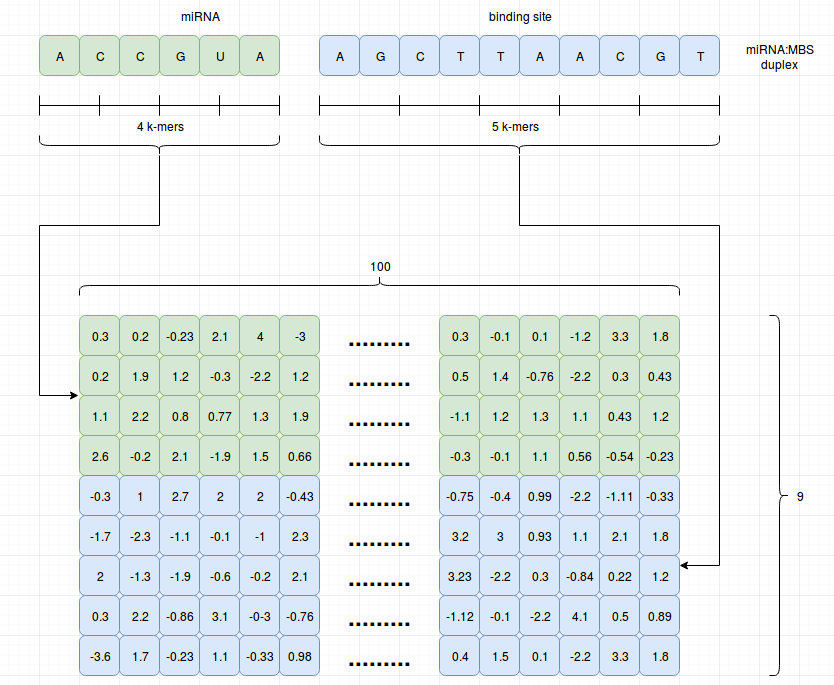
\includegraphics[width=\textwidth, height=0.4\textheight]{Figures/dna_embedding}
	\caption{\textbf{Sequence Embedding.} In green the miRNA sequence is split into 4 k-mers each mapped in a 100-dimension vector. In blue the same is done with miRNA binding site which is divided into 5 k-mers. The concatenation of the 9 resulting vectors is the matrix distributed representation of the duplex.}
	\label{fig:dna_embedding}
\end{figure}

With this representation, we believe the best base model to use for our task is represented by a convolutional neural network. 

\subsection{CNN architecture}
Once the baseline model has been chosen, one must proceed with its implementation selecting the best possible design. This step can be very tricky, especially when dealing with convolutional networks.  In fact, according to the complexity of the architecture and the representation of the available data, a CNN may require a long training time, with a great number of epochs. This makes the evaluation of the model design a complicated task: large validation errors and little improvements in the first few epochs does not always imply that the chosen architecture is wrong.   

For DeepMiRNA, the network was configured so that the number of inputs in the input layer was equal to the dimensionality of the encoded sequences,  while the output layer consisted of two softmax neurons. 

The architecture of our convolutional network is shown in figure \ref{fig:cnn} and it is mainly inspired to the CNN used in \cite{cnn_arch}. Given that our model must be trained on a relatively small dataset we decided to adopt a single level of convolutional feature map followed by a non-linear ReLU activation layer and a max pooling layer immediately preceding the output softmax neurons. 

\begin{figure}[hbt!]
	\centering
	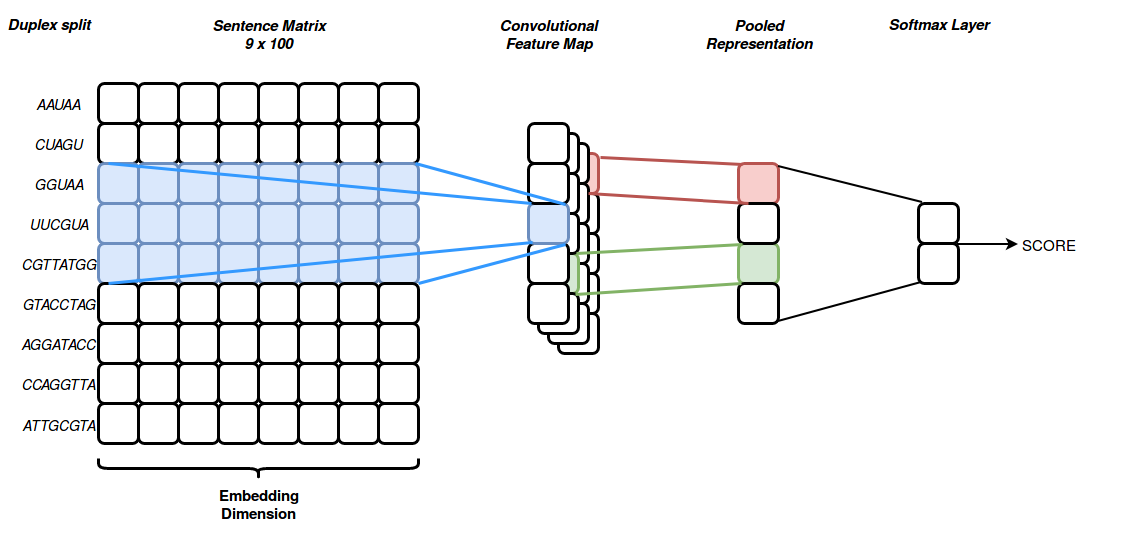
\includegraphics[width=\textwidth, height=0.4\textheight]{Figures/cnn_arch}
	\caption{\textbf{CNN architecture.} The input duplex is first split in 9 different length kmers to form the sentence matrix. The matrix is then fed into the convolutional network for prediction.}
	\label{fig:cnn}
\end{figure}     

For the compiling step required for the training stage, we selected the binary cross entropy loss function and we set the Adam optimizer with the same parameters used for the MLP network.

Despite showing discrete results in terms of accuracy and F1-score on the validation set composed of never seen miRNA:MBS examples, the CNN does not perform very well on the test set especially if compared to the feed-forward network. The main issue
concerns its scarce ability in correctly identifying negative miRNA:mRNA pairs. This fact, unfortunately, prevents this model from having a good generalization. We believe the main reason behind this, it is most likely due to the very small amount of negatively validated entries in the training set: issue that, instead, does not seem to affect the MLP model performance.

  

